\documentclass[thesis.tex]{subfiles}

\chapter{Bài toán xác minh người nói}

\section{Giới thiệu bài toán xác minh người nói}

Xác minh người nói (Speaker Verfication) là một trong hai ứng dụng lớn của nhận dạng người nói (Speaker Recognition). Trong phần này, đồ án sẽ giới thiệu về bài toán nhận dạng người nói và bài toán xác minh người nói.

\subsection{Nhận dạng người nói}

Nhận dạng người nói là quá trình tự động nhận dạng người đang nói bằng cách sử dụng thông tin độc nhất của người nói đó có trong tín hiệu giọng nói. Nhận dạng người nói được ứng dụng rộng rãi trong nhiều lĩnh vực khác nhau, tuy nhiên cũng gặp không ít khó khăn khi triển khai trong thực tế. Do vậy, nghiên cứu bài toán nhận dạng người nói rất được quan tâm bởi nhiều nhà khoa học trên thế giới. Một số ứng dụng của bài toán có thể kể đến như: (i) Bảo mật cho các hệ thống tài chính, ngân hàng: người dùng dùng giọng nói kết hợp với các lớp bảo mật khác cho xác thực để tăng tính bảo mật khi giao dịch. (ii) Tăng trải nghiệm khách hàng trong tổng đài chăm sóc khách hàng. (iii) Xác định danh tính tội phạm trong an ninh khi thu được dữ liệu giọng nói. (iv) Kết hợp với các hệ thống nhận dạng tiếng nói để xây dựng ứng dụng gỡ băng cuộc họp.

\subsection{Xác minh người nói}

Dựa vào ứng dụng, nhận dạng người được phân loại thành xác định người nói (Speaker Identitfication) và xác minh người nói (Hình \ref{fig:verification-identification}). Trong xác định người nói, một đoạn tiếng nói từ một người không xác định được phân tích và so sánh với biểu diễn giọng nói của những người đã biết. Người này được xác định là người có biểu diễn giọng nói phù hợp nhất với câu nói đầu vào. Trong xác minh người nói, một người lạ xác nhận một danh tính đã biết; đoạn tiếng nói của người này được so sánh với biểu diễn giọng nói của danh tính đang được xác nhận. Nếu điểm tương đồng đủ tốt, nghĩa là trên một ngưỡng nào đó, danh tính của người lạ được chấp nhận. Ngưỡng cao khiến những kẻ mạo danh khó được chấp nhận bởi hệ thống, nhưng có nguy từ chối nhầm người dùng hợp lệ. Ngược lại, ngưỡng thấp cho phép chấp nhận người dùng hợp lệ một cách nhất quán, nhưng có nguy cơ chấp nhận những người giả mạo. Xác minh người nói được ứng dụng phổ biến hơn xác định người nói do nhu cầu và dễ thực hiện hơn về mặt tính toán (một phép so sánh so với N phép so sánh trong xác định người nói). Thông thường, cải tiến trong một trong hai bài toán có thể được áp dụng sang bài toán còn lại.

\begin{figure}[h]
    \centering
    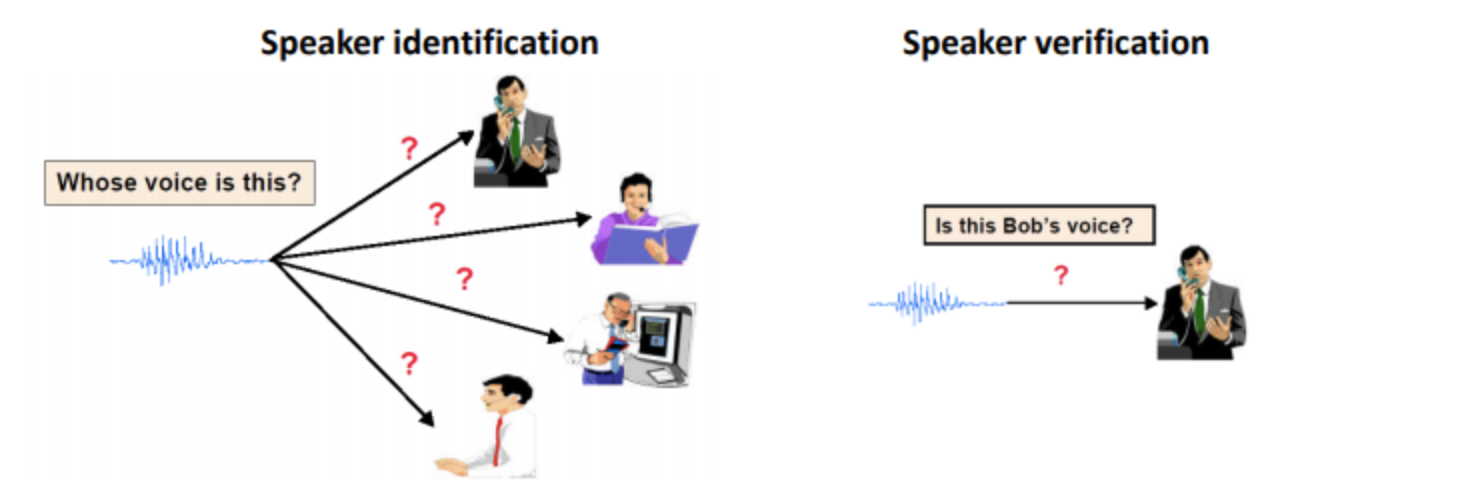
\includegraphics[width=1.0\textwidth]{images/identification-verification.png}
    \caption{Xác định người nói và xác minh người nói \protect\footnotemark.}
    \label{fig:verification-identification}
\end{figure}
\footnotetext{https://wiki.aalto.fi/display/ITSP/Speaker+Recognition+and+Verification}

Xác minh người nói có tiềm năng ứng dụng trong xác thực cá nhân, bao gồm xác minh thẻ tín dụng, truy cập bảo mật qua điện thoại (di động, Internet) trong các trung tâm cuộc gọi. Ngoài ra, xác minh người nói còn được ứng dụng trong an ninh có thể kể đến như nhận dạng nghi phạm qua giọng nói, truy cập vào toà nhà hay các biện pháp an ninh quốc gia chống khủng bố bằng cách sử dụng giọng nói làm bảo mật cho các ứng dụng quan trọng. Với việc bảo mật thông tin cá nhân trở thành một vấn đề nóng hổi trong xã hội, các công ty Internet cũng có thể sử dụng xác minh người nói để ngăn chặn khả năng gian lận danh tính.

Thông thường, hệ thống xác minh người nói được chia thành 3 pha (Hình \ref*{fig:overall-system}):

\begin{itemize}
    \item Pha 1: Phát triển (Development). Trong pha này, mô hình có khả năng biểu diễn đặc trưng người nói được huấn luyện và tối ưu trên một cơ sở dữ liệu lớn các đoạn tiếng nói từ một nhóm nhiều người nói khác nhau.
    \item Pha 2: Ghi danh (Enrollment). Trong pha ghi danh, biểu diễn của người dùng mới được trích xuất bằng mô hình phát triển ở pha 1 và lưu trữ trong cơ sở dữ liệu để phục vụ cho pha 3.
    \item Pha 3: Kiểm tra (Testing). Trong pha này, được cung cấp danh tính đầu vào, hệ thống chỉ so sánh đoạn tiếng nói đầu vào và đoạn của danh tính trong hệ thống để đưa ra quyết định.
\end{itemize}

\begin{figure}[h]
    \centering
    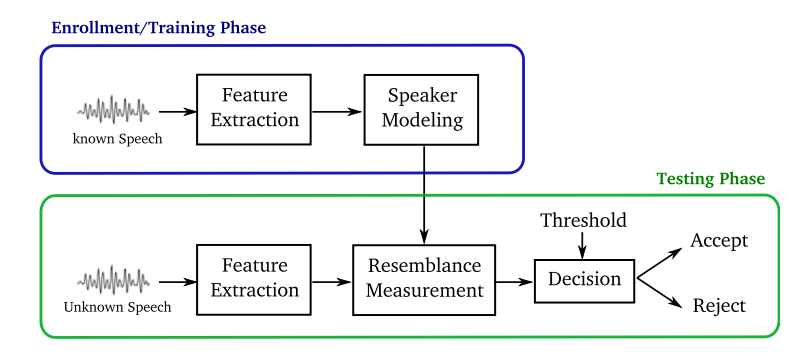
\includegraphics[width=1.0\textwidth]{images/overall-system.png}
    \caption{Tổng quan hệ thống xác minh người nói \protect\footnotemark.}
    \label{fig:overall-system}
\end{figure}
\footnotetext{https://wiki.aalto.fi/display/ITSP/Speaker+Recognition+and+Verification}

Trong thực tế, hiệu năng của hệ thống xác minh người nói bị suy giảm do sự khác biệt của các kênh và phiên giữa tín hiệu giọng nói trong pha ghi danh và pha kiểm tra. Các yếu tố làm ảnh hưởng tới tín hiệu giọng nói bao gồm:

\begin{itemize}
    \item Sử dụng các loại micrô khác nhau khi thu tín hiệu đăng ký và kiểm tra.
    \item Điều kiện tiếng ồn và độ vang của môi trường.
    \item Sự khác biệt trong giọng nói của người nói ở các giai đoạn khác nhau của độ tuổi, sức khoẻ, phong cách nói và trạng thái cảm xúc.
    \item Các kênh truyền như các loại điện thoại di động khác nhau, micrô, giao thức truyền tín hiệu giọng nói qua Internet có thể làm thay đổi giọng.
\end{itemize}

Dựa vào sự tương đồng của các câu nói đầu vào, phương pháp giải quyết bài toán xác minh người nói có thể được chia thành hai loại: phụ thuộc văn bản (Text-Dependent Speaker Verification - TDSV) và không phụ thuộc văn bản (Text-Independent Speaker Verification - TISV). Các hệ thống TDSV yêu cầu người nói cung cấp các đoạn tiếng nói có nội dung thuộc một tập các từ hoặc câu được định sẵn; nội dung các câu nói phải được giữ nhất quán trong cả quá trình huấn luyện và xác minh. Ngược lại, TISV không yêu cầu người dùng phải thu theo bất cứ một văn bản nào. Với các đoạn tiếng nói ngắn, các hệ thống TDSV đã có thể đạt được hiệu suất nhận diện cao, trong khi TISV yêu cầu các câu nói dài hơn và một lượng lớn dữ liệu để huấn luyện các mô hình đáng tin cậy và đạt được hiệu suất tốt. Do sự tiện lợi của TISV so với TDSV, các hệ thống sử dụng trong thương mại hiện nay phần lớn là TISV.

\section{Nghiên cứu xác minh người nói trên thế giới} \label{related-works}
Nghiên cứu về xác minh người nói hay nhận dạng người nói trên thế giới đã bắt đầu từ những năm 1980; các mô hình cho xác minh người nói có thể được phân vào 2 nhóm: các mô hình thống kê và các mô hình học sâu.

\subsection{Mô hình thống kê}
Mô hình xác minh người nói và nhận dạng người nói tự động đầu tiên được đề xuất năm 1995 bởi Reynolds và cộng sự \cite{reynolds1995robust}. Phương pháp sử dụng trong nghiên cứu là mô hình Gaussian hỗn hợp (Gaussian Mixture Model - GMM). GMM là tổng hợp của nhiều hàm mật độ xác suất Gaussian, thường được dùng để mô hình dữ liệu đa biến. Sử dụng GMM để mô hình hoá đặc trưng của một người nói thu được hàm mật độ xác suất phụ thuộc vào người nói. Xác suất tương đồng giữa GMM của một người nói và một câu nói bất kì có thể được tính nhờ hàm mật độ xác suất này. Với một ứng dụng xác minh người nói đơn giản, trong pha ghi danh, một GMM được tính toán cho mỗi người trong cơ sở dữ liệu. Trong pha kiểm tra, câu nói được cung cấp được so sánh với GMM của danh tính mà người nói cung cấp. Nếu điểm tương đồng vượt qua một ngưỡng nhất định, danh tính này được chấp nhận.

Một thời gian sau đó, nhận thấy phương pháp GMM yêu cầu quá nhiều dữ liệu cho mỗi người nói, phương pháp GMM-UBM ra đời. Về cơ bản, UBM (mô hình nền phổ quát - Universal Background Model) là một GMM lớn mô tả phân phối không phụ thuộc vào người nói từ đặc trưng tiếng nói của tất cả người nói trong cơ sở dữ liệu. Tại pha ghi danh, UBM được thích ứng cho mỗi người nói sử dụng phương pháp thích ứng Baysian. Phương pháp GMM-UBM cho kết quả vượt trội so với việc huấn luyện GMM độc lập cho mỗi người nói từ đầu với một lượng dữ liệu ít hơn.

Một trong những vấn đề với xác minh người nói là dữ liệu giọng nói huấn luyện và kiểm tra có thể có thời lượng khác nhau. Điều này đòi hỏi sự so sánh của hai câu nói có độ dài khác nhau. Do đó, một trong những nỗ lực hướng tới việc xác minh người nói hiệu quả là có được biểu diễn với chiều cố định cho một câu nói duy nhất. Việc có được biểu diễn có chiều cố định cực kì hữu ích vì nhiều phương pháp phân loại khác nhau trong học máy có thể sử dụng các biểu diễn này để phân loại. 

Một giải pháp hiệu quả để có được vectơ chiều cố định từ câu nói có thời lượng thay đổi là GMM siêu vec-tơ (Supervector), về cơ bản là một vectơ lớn thu được bằng cách ghép các tham số trong mô hình GMM. Phương pháp ứng dụng siêu vec-tơ trong xác minh người nói được đề xuất năm 2003 bởi Kenny và cộng sự \cite{kenny2003new}, thúc đẩy nhiều phương pháp thích ứng mô hình mới. Cộng đồng nhận ra các siêu vec-tơ với chiều lớn là một nền tảng tốt để thiết kế các phương thức loại bỏ thông tin về kênh và phiên như đã nói trong mục trước để có được vec-tơ biểu diễn người nói hiệu quả hơn. Các phương pháp thống trị hoạt động trên không gian siêu vec-tơ dựa trên phân tích nhân tố (Factor Analysis) và máy vec-tơ hỗ trợ (Support Vector Machine). Các phương pháp sử dụng GMM-UBM và siêu vec-tơ vẫn được coi là phương pháp hiện đại nhất cho bài toán xác minh người nói cho đến nửa cuối của những năm 2010 với sự phát triển mạnh mẽ của học sâu.

\subsection{Mô hình học sâu}
Các mô hình học sâu hiện đại giải quyết bài toán xác minh người nói thường gồm ba phần chính (Hình \ref{fig:model-architecture}):

\begin{itemize}
    \item Một mạng nơ-ron làm công cụ trích xuất biểu diễn người nói cho một khung đặc trưng tiếng nói.
    \item Lớp tổng hợp dữ liệu: lớp này sử dụng biểu diễn của các khung giọng nói từ mạng nơ-ron để tổng hợp ra một vec-tơ duy nhất đại diện cho đoạn tiếng nói đầu vào.
    \item Một hàm mất mát để tối ưu toàn bộ mô hình.
\end{itemize}

\begin{figure}[h]
    \centering
    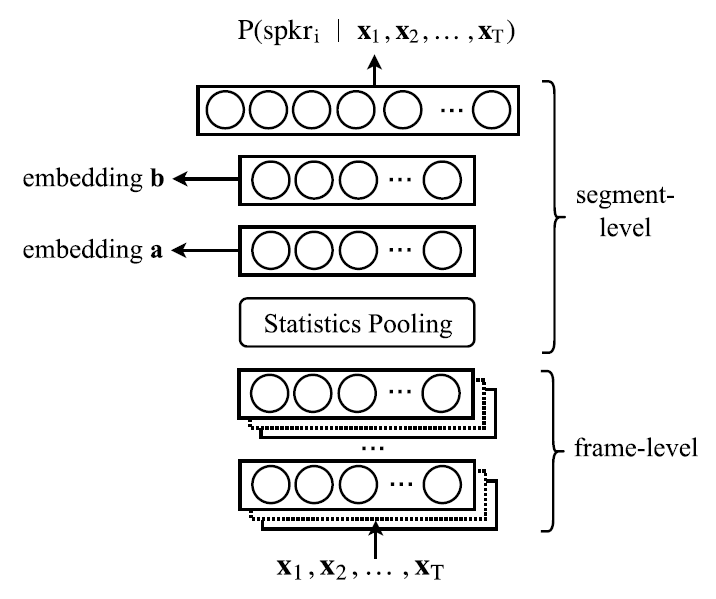
\includegraphics[width=0.7\textwidth]{images/x-vector.png}
    \caption{Kiến trúc mô hình xác minh người nói với học sâu \cite{snyder2018x}.}
    \label{fig:model-architecture}
\end{figure}

Trong pha kiểm tra, mạng nơ-ron và lớp tổng hợp dữ liệu được sử dụng để tạo ra vec-tơ biểu diễn của đoạn tiếng nói kiểm tra. Hàm mất mát chỉ được sử dụng trong pha phát triển, và bị loại bỏ trong pha kiểm tra và pha ghi danh.

Phần lớn các nghiên cứu học sâu cho xác minh người nói hướng tới cải thiện hệ thống qua nâng cao hiệu quả của lớp tổng hợp dữ liệu và hàm mất mát. Về mạng nơ-ron trích xuất đặc trưng, các nghiên cứu chủ yếu sử dụng các mạng xương sống thành công trong các bài toán khác như phân loại hình ảnh (Ví dụ: mạng VGG \cite{simonyan2014very} và mạng ResNet \cite{he2016deep}) và nhận dạng tiếng nói (mạng TDNN \cite{waibel1989phoneme} và mạng LSTM \cite{hochreiter1997long}).

Sự thành công và hiệu quả của học sâu cho bài toán xác minh người nói trong tiếng Anh đến từ hai yếu tố. Thứ nhất, các kiến trúc mô hình, lớp tổng hợp dữ liệu và hàm mất mát được nghiên cứu kỹ lưỡng để phù hợp hơn với dạng dữ liệu và bài toán từ đó cải thiện hiệu năng. Thứ hai, các bộ dữ liệu người nói cực lớn như VoxCeleb \cite{nagrani2020voxceleb} và SITW \cite{mclaren2016speakers} được phát triển và mở công khai cho cộng đồng nghiên cứu sử dụng. Các nghiên cứu gần nhất về học sâu cho xác minh người nói không phụ thuộc văn bản đạt kết quả rất tốt xấp xỉ 1\% EER trên tập VoxCeleb1 \cite{heo2020clova, desplanques2020ecapa}.

\section{Xác minh người nói trong tiếng Việt và vấn đề đặt ra} \label{vietnamese-speaker-recognition}
Ở Việt Nam trong những năm vừa qua, nhờ vào sự phát triển của ngành công nghệ thông tin cũng như sự phát triển mạnh mẽ của nền kinh tế đã tạo điều kiện nghiên cứu, phát triển và triển khai các ứng dụng công nghệ mang lại  nhiều lợi ích cho xã hội. Các ứng dụng trí tuệ nhân tạo như nhận dạng khuôn mặt, xác minh người nói cũng không nằm ngoài xu thế. Tuy nhiên, theo hiểu biết của tác giả, các nghiên cứu về xác minh người nói tiếng Việt hay dữ liệu công khai cho bài toán còn rất hạn chế.

Năm 2010, luận án tiến sĩ của TS. Ngô Minh Dũng \footnote{\href{http://luanan.nlv.gov.vn/luanan?a=d\&d=TTcFabDIJkxi2010.1.5\#}{http://luanan.nlv.gov.vn/luanan?a=d\&d=TTcFabDIJkxi2010.1.5\#}} nghiên cứu giải quyết bài toán xác minh người nói tiếng Việt phụ thuộc văn bản. Nghiên cứu xây dựng cơ sở dữ liệu với 150 người nói với 17 âm tiết khác nhau bao gồm 10 âm tiết số và 7 âm tiết khác để thử nghiệm. Luận án sử dụng mô hình Gaussian  hỗn hợp nhằm mô tả phân phân bố tần số cộng hưởng của tuyến phát âm để mô tả người nói. Nghiên cứu \cite{haspeaker, 7054126} bởi các trường Đại học Sư phạm Huế, Đại học Sư phạm Kỹ thuật Hưng Yên và Đại học Bách khoa Hà Nội cùng giải quyết bài toán xác minh người nói phụ thuộc văn bản sử dụng mô hình Gaussian hỗn hợp. Nghiên cứu đầu tiên áp dụng học sâu cho bài toán xác minh người nói tiếng Việt phụ thuộc văn bản đạt 3.87\% EER được công bố tại hội nghị SoICT lần thứ 9 vào năm 2018 \cite{nguyen2018vietnamese}. Hiện tại chưa có nghiên cứu hay hệ thống thương mại nào cho xác minh người nói không phụ thuộc văn bản trong tiếng Việt.

Các mô hình xác minh người nói không phụ thuộc văn bản tuy thuận tiện khi sử dụng nhưng để xây dựng mô hình chất lượng tốt cần một lượng dữ liệu khổng lồ. Bộ dữ liệu VoxCeleb thường được sử để xây dựng các mô hình tiếng Anh VoxCeleb có hơn 7,000 danh tính khác nhau, hơn 1,000,000 đoạn giọng nói với tổng độ dài hơn 2,000 giờ. Bộ dữ liệu công khai duy nhất trong tiếng Việt phục vụ cho bài toán không phụ thuộc văn bản được xây dựng cho cuộc thi ZaloAI challenge \cite{ZaloAIChallenge} bao gồm 400 danh tính, 10,000 đoạn tiếng nói với tổng độ dài 8.7 giờ, ít hơn rất nhiều so với bộ dữ liệu tiếng Anh. Với lượng dữ liệu nhỏ, việc xây dựng mô hình chất lượng tốt cho tiếng Việt trở nên rất khó khăn.

Như đã đề cập trong mục này và các mục trước, xác minh người nói có tính ứng dụng cao và nhận được nhiều sự quan tâm từ cộng đồng nghiên cứu. Đối với xác minh người nói không phụ thuộc văn bản trong tiếng Việt, bộ dữ liệu phục vụ cho bài toán còn rất nhỏ và chưa có nghiên cứu về học sâu cho bài toán trong tiếng Việt. Do đó, mục tiêu của đồ án là xây dựng bộ dữ liệu và đề xuất mô hình cho bài toán TISV trong tiếng Việt.

\section{Định hướng giải pháp}
Để giải quyết việc thiếu hụt dữ liệu phục vụ cho huấn luyện mô hình, tác tác giả bổ sung dữ liệu danh tính bằng các bộ dữ liệu nhận dạng tiếng nói là VIVOS, VLSP và CommonVoice. Ngoài ra nhận thấy bộ dữ liệu còn nhiều lỗi, tác giả cũng xây dựng một bộ làm sạch dữ liệu dựa trên biểu diễn người nói từ mô hình giúp loại bỏ các đoạn tiếng nói không hợp lệ, loại bỏ hay hợp nhất danh tính dễ dàng hơn từ đó tăng chất lượng bộ dữ liệu.

Trong khuôn khổ đồ án, tác giả tập trung vào thử nghiệm các kĩ thuật huấn luyện mô hình học sâu cho xác minh người nói không phụ thuộc văn bản trong tiếng Việt.

\section{Bố cục đồ án}
Trong chương 1, tác giả đã giới thiệu tổng quan về bài toán xác minh người nói, thảo luận về tình hình phát triển xác minh người nói trong tiếng Việt. Phần còn lại của đồ án được tổ chức như sau.

Chương 2 trình bày về cơ sở lý thuyết về học máy và học sâu, và phương pháp trích xuất đặc trưng âm học từ tín hiệu giọng nói.

Chương 3 trình bày về mô hình cơ sở sử dụng trong đồ án, các giải pháp đề xuất để huấn luyện mô hình một cách hiệu quả cùng với các nghiên cứu liên quan.

Trong chương 4, đồ án mô tả chi tiết phương pháp xây dựng bộ dữ liệu, phương pháp thực nghiệm và đánh giá kết quả thu được.

Chương 5 tổng kết các kết quả đạt được và định hướng phát triển trong tương lai.